\documentclass[a4paper,11pt]{report}
    \usepackage[utf8]{inputenc}
    \usepackage[T1]{fontenc} 
    \usepackage[francais]{babel}
    \usepackage{amsmath}
    \usepackage{amssymb}
    \usepackage{graphicx}
    \usepackage{color}
    \usepackage{hyperref}
    \usepackage[left=2cm,right=2cm,top=2cm,bottom=2cm]{geometry}
\usepackage{mathrsfs}
    \title{Application de chiffrement homomorphe a l'apprentissage automatique}

\author{BENISSA Sami\quad:\quad Université Paris 8}


\date{8 septembre 2017}
\begin{document}
%\begin{figure}
%\includegraphics[scale=1]{paris_8.png} 
% \end{figure}
\maketitle
\section{Remerciements}
\newpage
\section{Introduction}
\newpage
\section{Présentation de l’entreprise}
\newpage
\newpage

\section{objectif du stage}
Le But de  stage était de concevoir une application d'apprentissage automatique a partir des données chiffrées en utilisant un schéma de chiffrement homomorphe.\newline
Ce type d'application peut servir dans les domaines ou on veut appliquer de calcul sur des données privées.\newline
Par exemple chaque jour on voit sortir des applications d'apprentissage automatique dans le domaine médical mais la question est qu'on peut fournir le meme servir en gardant la confidentialité sur les informations des patients.\newline
La prémière étape durant la periode de stage l'objectif c'était de faire l'Etat de l'art sur les différents cryptosystème de chiffrerment homomorphe et de bien comprendre le concept de machine learning.\newline
La deuxième étape le but c'était d'implementer des algorithmes de machine learning sur des données clair afin de concevoir un modèle et régarder les différents métriques qu'il faut prendre en compte pour analyser l'efficacité du modèle.\newline
La dernière étape c'était pour implementer les memes algoritmes sur des données chiffrées et d'evaluer la différence par rapport au résultat obtenu a partir des algorithmes implementer dans la deuxième partie.\newline
\section{Etat de l'art} 
\subsection{chiffrement partiellement homomorphe}
Un cryptosystème est considéré partiellement homomorphic s'il commute 
\textit{definition : } On dira d’un cryptosystème est partiellement homomorphe 
\subsection{chiffrement complètement homomorphe}
\subsection{Quelques Applications de chiffrement homomorphe a l'apprentissage automatique}
Il est devenu possible de déléguer l'exécution d'un algorithme d'apprentissage à un service informatique tout en conservant la confidentialité des données. \newline
Avant de commencer à décrire les travaux effectués dans cette direction. Il est important de parler des différentes phases qui compose un algorithme d'apprentissage automatique.\newline
Le machine learning se décompose en 2 étapes:\newline
\underline{Une phase d’entraînement }:\newline on apprend sur une partie des données après choisir le modèle mathématique le plus adapté.\newline 
\underline{Une phase d'inférence ou de validation} :\newline	 on teste sur la seconde partie de données et mésurer le taux de réussite de notre modèle .\newline
Parmis les travaux on peut cité :\newline
\textit{Cryptonets } : Dans ce projet on trouve l'application des réseaux de neurones sur des données chiffrée. \newline
Dans cette application la phase d'apprentissage a été effectué sur des données clair  afin d'obtenir le modèle qui va servir dans la phase d'inférence, et ce dernier a été éffectué sur des données chiffrées.    
\textit{Biomedical Applications } :
\newpage
\section{chiffrement completement homomorphe}
Le chiffrement homomorphe permet de réaliser des calculs sur des données chiffrées générant un résultat chiffré qui lorsqu'il est déchiffré, correspond au résultat des opérations effectuées sur le texte en clair. 
\subsection*{les réseaux euclidiens}
\subsubsection*{Généralités sur les réseaux euclidiens}
\subsubsection*{\textcolor{red}{L'algorithme LLL}}
\subsubsection*{Réseau et cryptographie}
\subsection*{cryptosysteme completement homomorphe}
\subsubsection*{cryptosysteme BGV}
\subsubsection*{\textit{Schéma de  Fan et Vercauteren}}
Dans cette partie le vais présenter le schéma de Fan et Vercauteren\newline
Dans cette partie je vais présenter le schéma de FV qui a été utiliser dans SEAL avec quelques modifications.\newline
\newline
\vspace{100\baselineskip}
\newcommand{\bigslant}[2]{{\raisebox{.2em}{$#1$}\left/\raisebox{-.2em}{$#2$}\right.}}
\begin{tabular}{|c|c|c|}

\hline
 Paramètre& Description & Nom dans SEAL \\
\hline
$q$ & Modulus in the ciphertext space (coefficient modulus) & coeff\_modulus  \\
\hline
$t$ & Modulus in the plaintext space (plaintext modulus) & plain\_modulus \\
\hline
n & Une puissance de 2 &   \\
\hline
$(x^{n}+1)$ & polynôme de degré n  & poly\_modulus  \\
\hline
$R$ & L'anneau $\bigslant{\pmb{\mathbb{Z}}[X]}{(x^{n}+1)}$ & 8  \\
\hline
$R_a$ & L'anneau $\bigslant{\pmb{\mathbb{Z_a}}[X]}{(x^{n}+1)}$ avec descoefficients reduit modulo a &  \\
\hline
$w$ & Base dans laquel les messages chiffré durant la relinearization & 12 \\
\hline
7 & 7 & 14 \\
\hline
8 & 8 & 16 \\
\hline
9 & 9 & 18 \\
\hline
10 & 10 & \\
\hline

\end{tabular}
\newline
\textbf{\textit{ Espace de texte clair .}}\newline

L'espace de message clair est $R_t$ c'est-à-dire des polynômes de degré inférieur à n avec des coefficients modulo t. on utilise également la structure de l'anneau $R_t$, par exemple, un produit de deux polynômes en texte clair deviennent le produit de deux polynômes avec $x^n = -1$.\newline
Si on veut chiffrer une information on doit passer par un processus d'encodage, par exemple, si on veut chiffrer un entier ce dernier doit etre transformer en un polynome de $R_t$. le processus d'encodage et de décodage sera détaillé plus tard.\newline 
\textbf{\textit{ Espace de texte chiffré .}}\newline
Les messages chiffrés dans le schéma de FV ces sont des vecteurs  des polynomés de taille au mois égale a deux, et qui grandissent en taille avec la multiplication et qui va étre détailler au moment de présenter le processus de chiffrement. 
\subsection*{Algorithme}
Le schéma de Fan et Vercautreen contient sept algorithmes : \newline
 \begin{description}
 \item[SecretKeyGen$(\lambda)$:]  on choisit aléatoirement s dans $R_2$ et on prend $sk=s$.
 \item[PublicKeyGen$(sk)$ :] .
 \item[EvaluationKeyGen $(sk, w)$:] $for\quad i\in \{1......l\}$ on choisti $a_i\xleftarrow{}{}R_q$,$e_i\xleftarrow{}{}\chi.$\newline
 $$evk = ([-(a_is+e_i)+w^is^2]_q, a_i)$$
 \item[Encrypt $(pk, m)$:] Pour $m \in R_t$ et $Pk = (p_0, p_1)$ échantillonner, $u\xleftarrow{}{} {R_2}$, et $e_1,e_2 \xleftarrow{}{} \chi$.
 \newline et on calcul $Enc(m) = ct = ([\Delta m + p_0 u + e_1]_q, [p_1 u + e_2]_q).$
 \item[Decrypt $(sk, ct)$:] on a $s = sk $, soit $c_0 = ct[0]\quad et\quad c_1 = ct[1]$, on a $Dec(ct) = [\lfloor\dfrac{t}{q}[c_0 + c_1 s]_q\rceil]_t$
 \item[Add  $(ct_0, ct_1)$:]  $ct_0 + ct_1 = (ct_0[0] + ct_1[0], ct_0[1] + ct_1[1])$.
 \item[Multiply $(ct_0, ct_1)$:] on clacul, \newline
 $$c_0 = [\lfloor\dfrac{t}{q}ct_0[0]ct_1[0]\rceil]_q.$$
 $$c_1 = [\lfloor\dfrac{t}{q}(ct_0[0]ct_1[1] + ct_0[1]ct_1[0])\rceil]_q.$$
 $$c_2 = [\lfloor\dfrac{t}{q}ct_0[1]ct_1[1]\rceil]_q .$$ 
 aprés on exprime $c_2 $ dans la base $w$ $$c_2 = \sum_{i=1}^{l}c_2^{(i)}w^i.$$
 $$c_0^{'} = c_0 + \sum_{i=1}^{l}evk[i][0]c_2^{(i)} .$$
 $$c_1^{'} = c_1 + \sum_{i=1}^{l}evk[i][1]c_2^{(i)} .$$
 et donc le produit de deux chifrés sera $(c_0^{'}, c_1^{'}).$
  \end{description}

\newpage
\section{Apprentissage automatique}
\subsection*{definition}
L'apprentissage automatique (machine learning en anglais) est une discipline consacré a l'analyse des données. cette discipline nous permet de créer des connaissances automatiques a partir des données brutes, cela consciste a la mise en place des algorithmes (ou modèle) qui vont etre exploiter pour prendre des décisions.\newline
le schéma suivant montre le mode de fonctionnement d'un modèle en machine learning.\newline
\hspace*{4cm}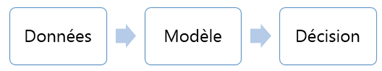
\includegraphics[scale=1]{m_learning.png} 
 \begin{enumerate}
 \item a partir des données on construit le modèle.
 \item Le modèle permet de prendre des décisions.
 \item On se sert du modèle sur de nouvelles données afin de prendre des décisions.
 \end{enumerate}
\subsection{Les données}
les données sont appelées échantillons, en machine learning ils sont souvent présenter sous fourme des vecteurs.\newline
$x=(x_1, x_2,.............,x_p).$\newline
où p est le nombre de coordonnées aussi appelé nombre d’attributs.\newline
En machine learning on a deux types des données :\newline
\newline
\textbf{Les données labélisées :} on donne à l’algorithme un certain nombre d’exemples (input) sur lesquels apprendre, et ces exemples sont « labellisés », c’est-à-dire qu’on leur associe un résultat désiré (output). L’algorithme a alors pour tâche de trouver la loi qui permet de trouver l’output en fonction des inputs.\newline
\newline 
\textbf{Les données non-labélisée :} définition2.
\subsection{La décision} 
On distingue deux types des décisions pour les algorithmes en machine learning. \newline
\textbf{Sorties catégorisées ou discrètes :} le nombre de sorties possible est fini. Dans ce cas, les sorties possibles sont appelées classes\newline
\textbf{Sorties non-catégorisées ou continues :} le nombre de sorties possible est infini dont la sortie de l'algorithme y est dans $R$ .\newline
\hspace*{5cm}{}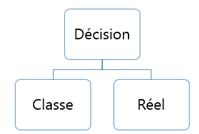
\includegraphics[scale=1]{classifictation_vs_regression.png}
\subsection{types d'apprentissages}
il y a deux pricipaux systèmes d'apprentissage qui définissent les différents modes de fonctionnement de machine learning.\newline
\title L’apprentissage supervisé ou analyse discriminatoire\newline
\title L’apprentissage non-supervisé ou clustering
\subsection{Algorithmes utilisés}
\newpage
\section{Implementation}
\subsection*{Regression Lineaire}
La regression linéaire est une modélisation linéaire qui permet de fournir des prédictions a partir des informations provenant du passé, 
Dans ce modèle on établi une relation entre une ou plusieurs variables explicatives $(x_1,x_2,..........,x_n)$ et une variable expliquée souvent noté par $Y$.\newline
La fonction d'evaluation dans la régression lineaire est la suivante : \newline
$$Y =h_{\theta}(x) = \theta^T = \sum_{i=1}^{n} \theta_ix_i $$\newline
ou $\theta_j (j=1................n)$ ces sont les paramètres du modèl qu'on devra estimer au moyen de techniques statistques parmis  lesquelles la descente de gradient stochastique.\newline
\newline
\subsubsection*{Algorithme de descente du gradient stochastique \textit{(stochastic gradient descent)}}.\newline
Cet algorithme permet de minimiser la fonction d'erreur (cost function) qui s'écrit sous la forme : \newline
$$J(\theta) = \dfrac{1}{2m}\sum_{i=1}^{m} (h_{\theta}^{x^{(i)}} - y^{(i)})^2$$\newline  
avec: \newline
$$h_{\theta}(x) = \theta^T = \sum \theta_ix_i $$
\newline
La descente de gradient stochastique premet de choisir les paramètres du modèl $\theta_i$ afin de minimiser la fonction d'erreur.\newline
Algorithme : \newline
\textit{inisialiser :} $\theta_i\quad pour\quad i=1 \quad jusqu'a\quad n$\newline
\textit{inisialiser : }$learning\_rate\quad(\alpha)$\newline
\textit{répéter}\{\newline 
\hspace*{1cm}\textit{pour j=1 jusqu'à m}\{
$$\theta_j := \theta_j - \alpha  \dfrac{1}{m}\sum_{i = 1}^{m} (h_\theta(x^{(i)}) - y^{(i)})x_j^{(i)} \quad(pour\, tout \, j)$$
\hspace*{1cm}\}\newline
\} 


\subsection*{Regression Logistique}
La regression logistique est une méthode statistique pour analyser un ensemble des données dans lequel il existe une ou plusieurs variables indépendantes qui servent a déterminer un résultat.\newline
L'objectif de la régression logistique est de trouver le meilleur modèle pour décrire le lien entre les vraiables explicatives et la variable dépondante ou la variable expliquée.\newline
Dans ce qui suit, nous noterons $Y$ la variable à prédire (variable expliquée), $X = (X_1, X_2, ..., X_J)$ les variables prédictives (variables explicatives). \newline
Dans le cadre de la régression logistique binaire, la variable $Y$ prend deux modalités possibles \{1, 0\}. Les variables $X_j$ sont exclusivement binaire. \newline
La fonction de prédiction dans la régression logistique est la suivante :\newline
$$h_{w,b}(x)=\dfrac{1}{1 + exp(-w^T x - b)}$$
ou $w_j$ : ces sont les paramètres du modèle.\newline
Pour l'estimation des paramètrs du modèle, on utilise l'algorithme de la descente de gradient stochastique qui sert a minimiser la fonction d'erruer :\newline
$$J(w,b) = \dfrac{1}{m}(\sum_{i=1}^{m}-y^{(i)}log(h_{w,b}(x^{(i)}))-(1-y^{(i)})log(1 - h_{w,b}(x^{(i)}))).$$\newline 
L'implementation de l'algorithme de la descente de gradient stochastique se fait de la meme façon que la régression linéaire.\newline
\textit{répéter}\{\newline 
\hspace*{1cm}\textit{pour j=1 jusqu'à m}\{
$$w_j := w_j - \alpha  \dfrac{1}{m}\sum_{i = 1}^{m} (h_{w,b}(x^{(i)}) - y^{(i)})x_j^{(i)} \quad(pour\, tout \, j)$$
$$ b := b - \alpha  \dfrac{1}{m}\sum_{i = 1}^{m} (h_{w,b}(x^{(i)}) - y^{(i)})$$
\hspace*{1cm}\}\newline
\} 
\subsection*{SEAL:Simple Encrypted Arithmetic Library}
\subsubsection*{présentation de la bibliotheque}
SEAL est une bibliothèque de chiffrement homomorphe qui est en cours de developpement par des chercheurs en cryptogreaphie a microsoft elle fait partie de logiciel libre, elle est écrit en C++11.
Un manuel détaillé pour l'utilisation de la version la plus récente de SEAL est disponible sur le lien \url{https://www.microsoft.com/en-us/research/publication/simple-encrypted-arithmetic-library-seal-v2-2/}. 
\textbf{différence entre l'implementation de SEAL et cryptosysteme Fan et Vercautreen}  \newline
En pratique, certaines opérations sont implementé d'une facon différente qui est plus générale.\newline
Dans cette partie on traite cette différence en détail.\newline

\textbf{\textit{message chiffré$(Ciphertext)$, message clair$(plaintext)$ dans SEAL.}}\newline
Les messages clairs dans SEAL c'est sont des élément de $R_t$ comme dans le cryptosysème Fan et Vercautreen,
Dans la version 2.2 les messages clairs sont présenter dans une classe Plaintext .\newline
Pour clarifier la généralisation des opérations FV, les messages chiffrés sont des vecteurs de taille qualconque et chaque composant chiffré correspond à une puissance de la clé secrète, Si on suppose que $ct = (c_0,..........,c_k)$ est un message chifré de taille $k+1$ alors,\newline
$c_0\quad correspond\quad à\quad s^0.$\newline
$c_1\quad correspond\quad à\quad s^1.$\newline
$c_k\quad correspond\quad à\quad s^k.$
\newline
 Dans SEAL les messages chiffré sont présenter dans une classe Ciphertext.\newline
 \textbf{Déchiffrement d'un message de taille quelconque.}\newline
soit $ct = (c_0, c_1, .........., c_k)$ une message chiffré de taille $k+1.$\newline
$Dec(ct) = Dec((c_0, c_1, .........., c_k)) = [\lfloor\dfrac{t}{q}[ct(s)]_q\rceil]_t = [\lfloor\dfrac{t}{q}[c_0 + c_1s+c_2s^2+.......,c_ks^k]_q\rceil]_t$\newline
Multiplication et addition de deux message dans SEAL\newline
\textit{Addition:}\newline
soient $ct_1$ et $ct_2$ deux message chifré telque,\newline
$ct_1 = (c_0,............,c_j)$, $ct_2 = (d_0,............,d_k)$
\newline
\textit{Addition : }\newline
\newline
$si\quad on\quad suppose\quad que\quad k\quad \leq \quad j\quad on\quad a \quad:$\newline
\newline
$Add(ct_1, ct_2) = (ct_1[0]+ct_2[0],ct_1[1]+ct_2[1],..............,ct_1[k]+ct_2[k])$\newline
\newline
\textit{Multiplication:}\newline
\newline
$Mult(ct_1, ct_2) = (C_1,C_2,............., C_{j+k})$ avec :\newline
$$C_m = [\lfloor\dfrac{t}{q}(\sum_{r+s=m}^{}c_rd_s)\rceil]_q.$$
\textit{Relinearization:}\newline
\newline
\textit{Autres opérations définies dans SEAL:}\newline
Toutes les opérations sont définies dans une classe Evaluator\newline
\begin{description}
 \item[Evaluator::negate :] permet d'evaluer la negation homomorphiquement,
 \item[Evaluator::add\_plain :] permet d'additioner Plaintext a un Ciphertext,
 \item[Evaluator::multiply\_plain :] multiplication entre Plaintext et Ciphertext,
 \item[Evaluator::sub\_plain :] soustraction entre Ciphertext et Plaintext,
 \item[Evaluator::multiply\_many :] multiplicatioon de plusieurs Ciphertext,
 \item[Evaluator::add\_many :] addition de plusieurs Ciphertext,
 \item[Evaluator::square :] elevation puissance 2,
 \item[Evaluator::exponentiate :] Elévation d'un message chiffré à une puissance qui est un nombre entier,
  \end{description}

\newpage
\end{document}